\section{Derivadas Parciais}

\subsection*{Motivação}
\begin{frame}[label=der-parciais]{Derivadas Parciais}
Suponha que a distribuição de temperaturas em uma placa quadrada é descrita pela função
\[f({\color{red}x},{\color{blue}y})=100-{\color{red}x^2}-{\color{blue}y^2}, \text{ com } -5\sqrt{2}\leq {\color{red}x},{\color{blue}y}\leq 5\sqrt{2},\]
onde a temperatura é medida em $^\circ C$ e o comprimento em metros.




\begin{center}
 \begin{minipage}{0.5\textwidth}
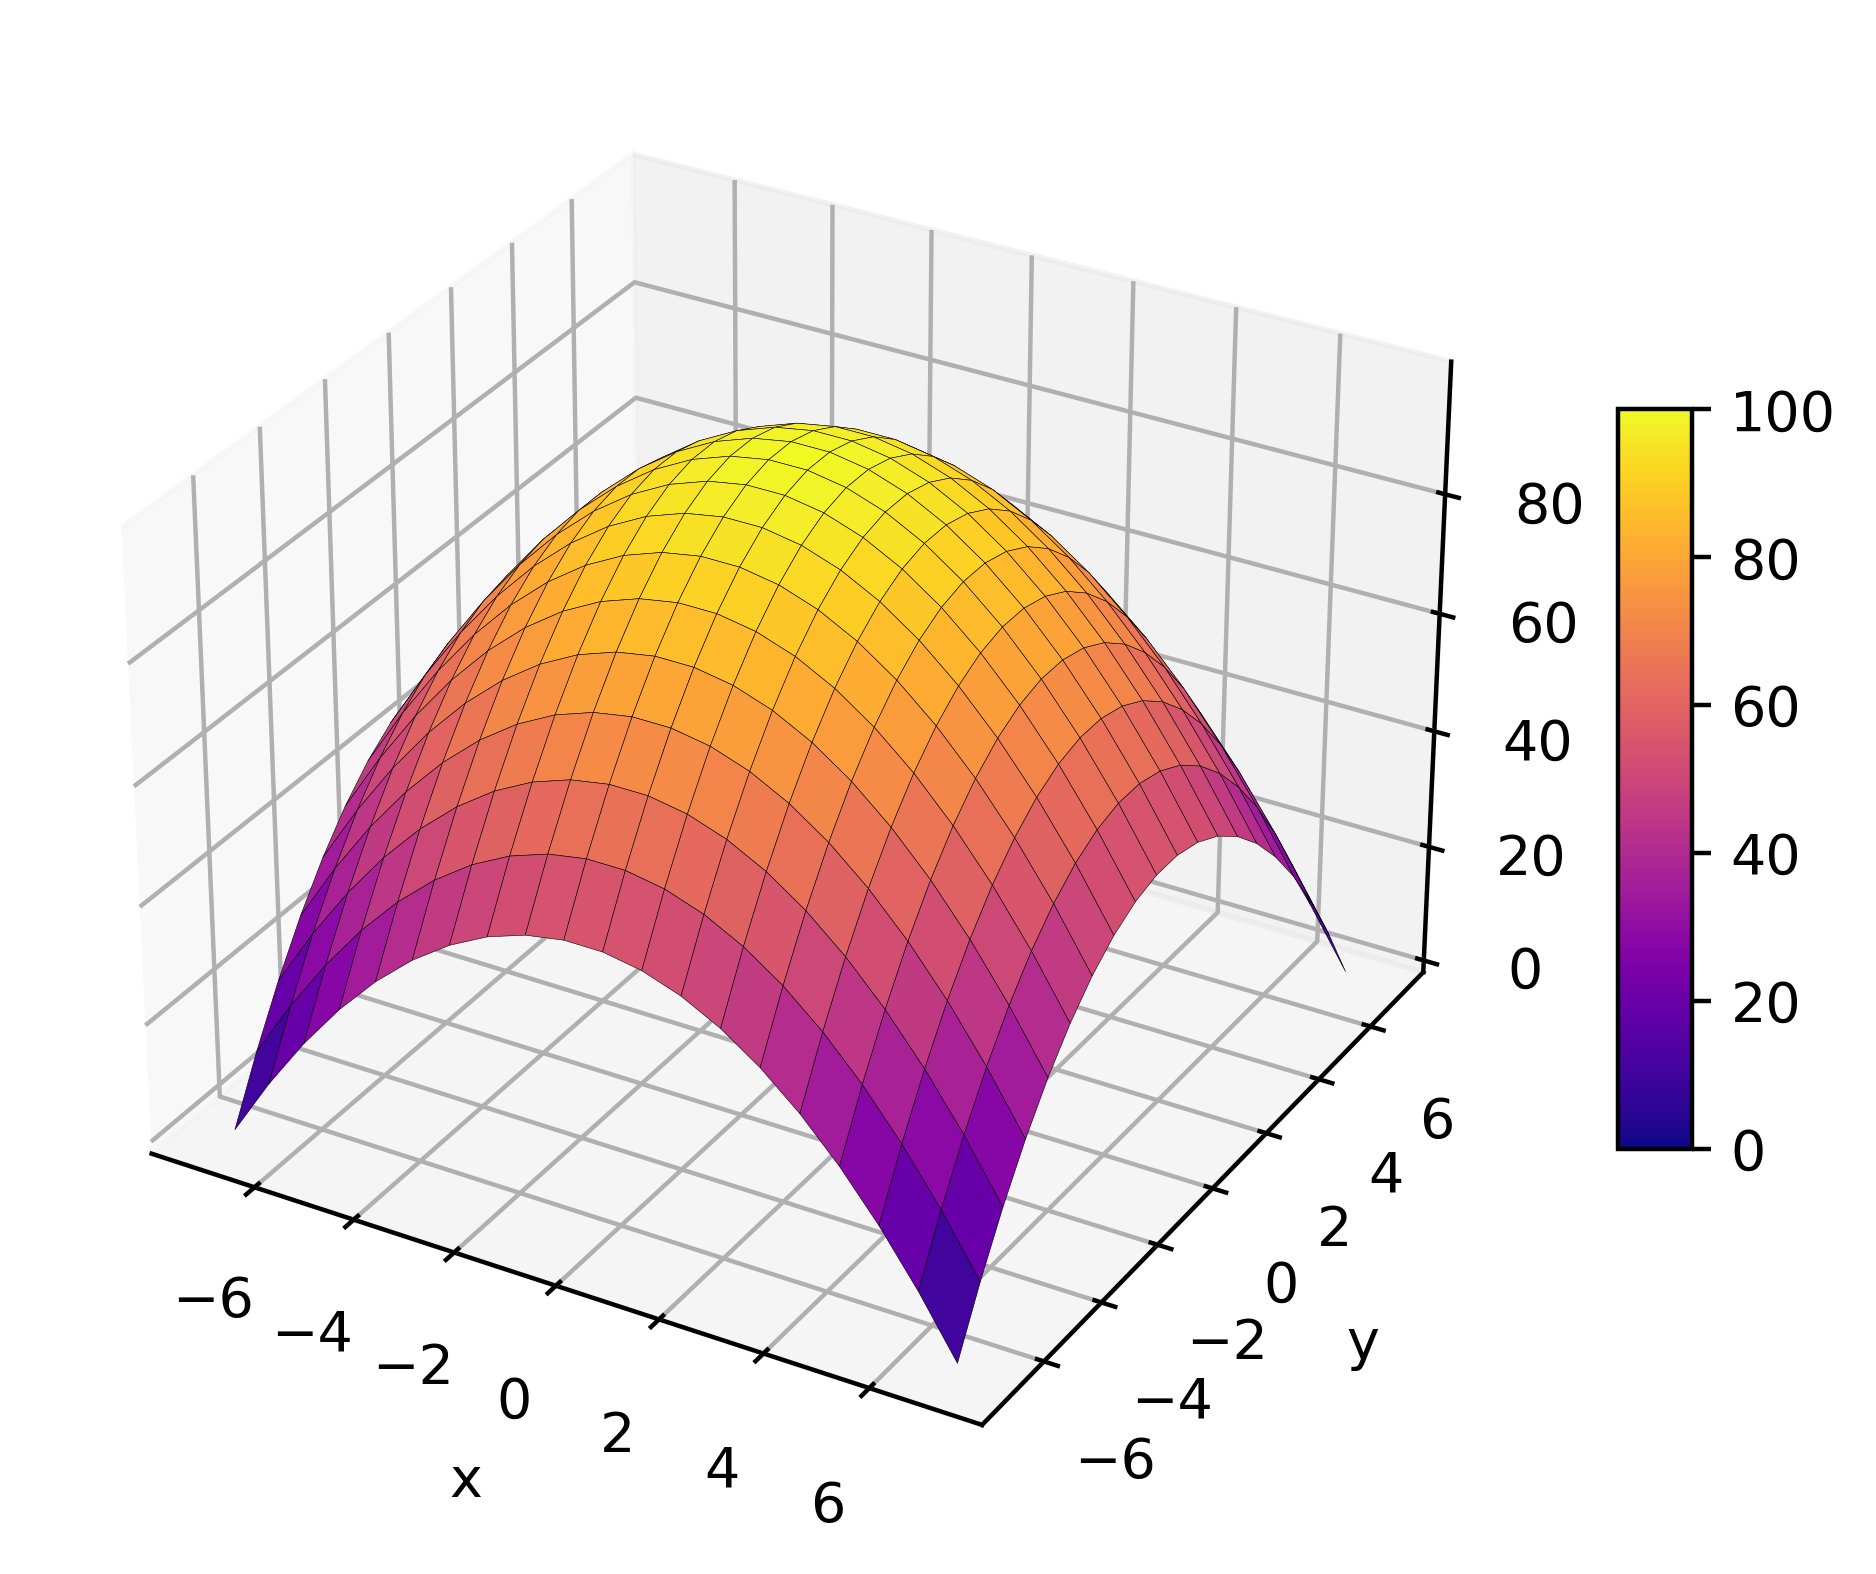
\includegraphics[scale=0.5]{figuras/der-parc2-1.png}
	 \end{minipage}
\begin{minipage}{0.4\textwidth}
	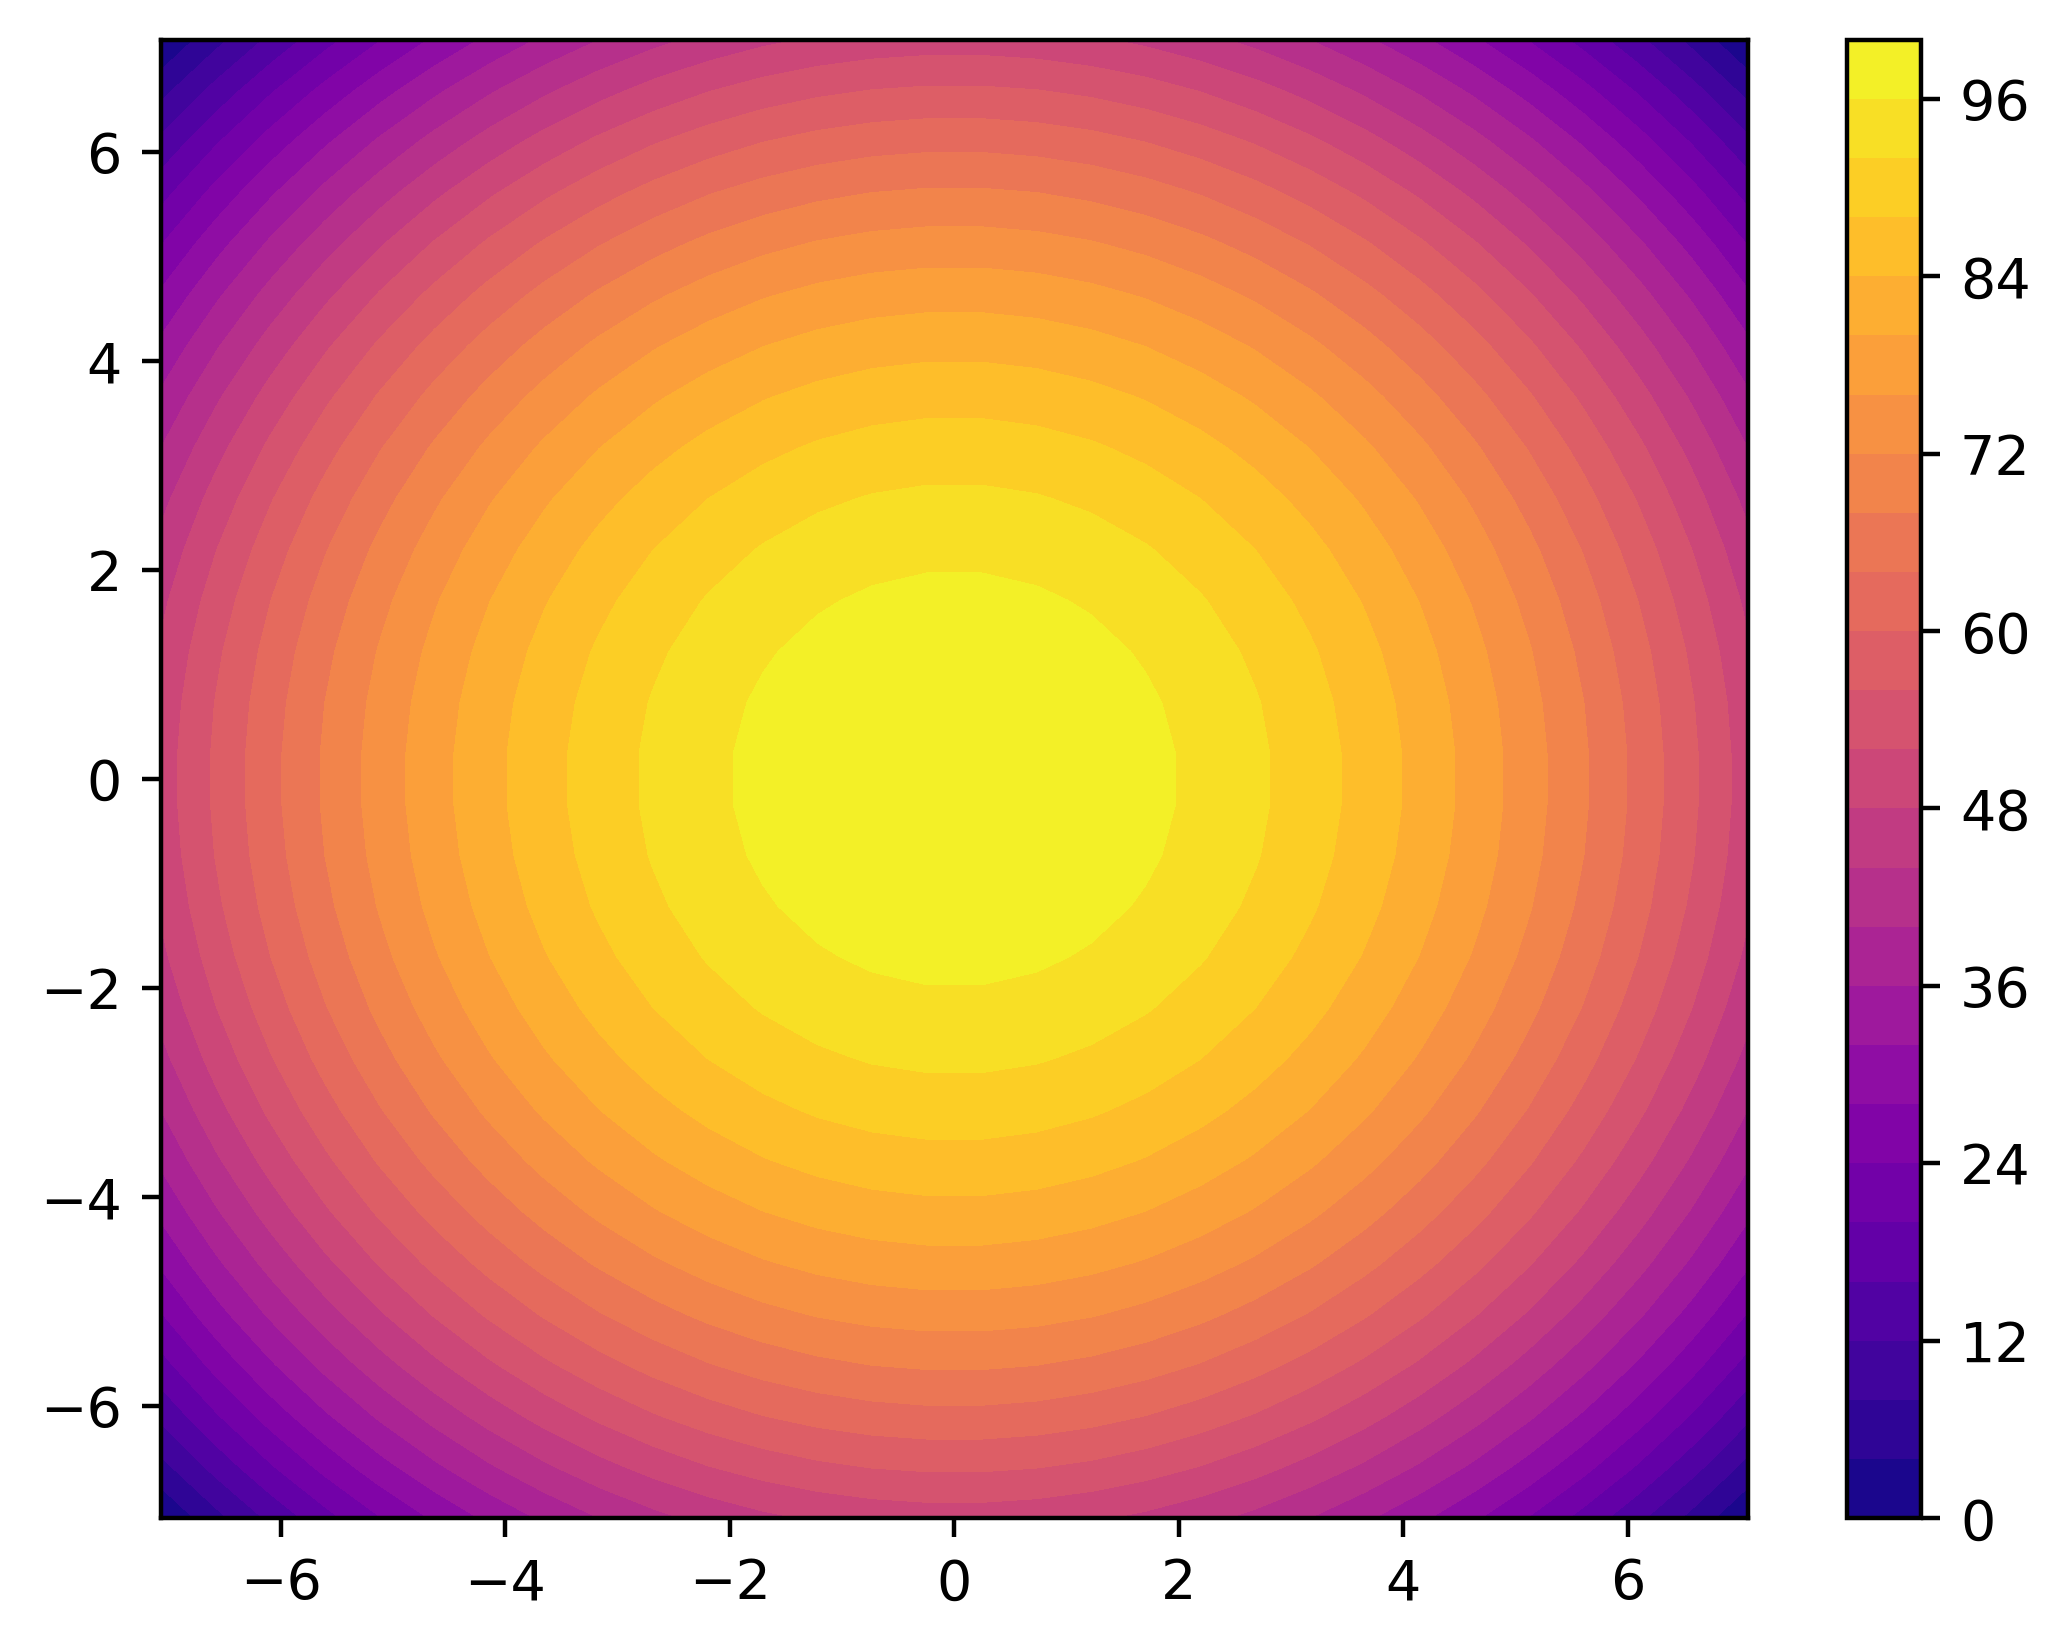
\includegraphics[scale=0.4]{figuras/der-parc2-1-nivel.png}
\end{minipage}
\end{center}


\end{frame}

%\begin{frame}[label=der-parciais]{Derivadas Parciais}
%Considere um paralelepípedo reto de altura {\color{blue}$y$} e base quadrada de lado {\color{red}$x$}.
%
%\begin{center}
%\begin{tikzpicture}
%\node at (0,0)
%{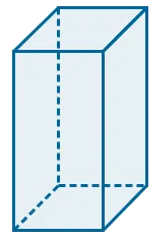
\includegraphics[scale=1]{figuras/paralelepidedo.png}};
%\node[color=red] at (-.2,-1.2) {$x$};
%\node[color=red] at (.7,-.8) {$x$};
%\node[color=blue] at (.8,.2) {$y$};
%\end{tikzpicture}
%\end{center}
%
%
% O volume deste paralelepípedo é dado pela função 
% \begin{minipage}{0.5\textwidth}
%\[V({\color{red}x},{\color{blue}y})={\color{red}x^2}{\color{blue}y}, \text{ com } {\color{red}x},{\color{blue}y}\geq 0.\]
% \end{minipage}
%\begin{minipage}{0.4\textwidth}
%\begin{center}
%	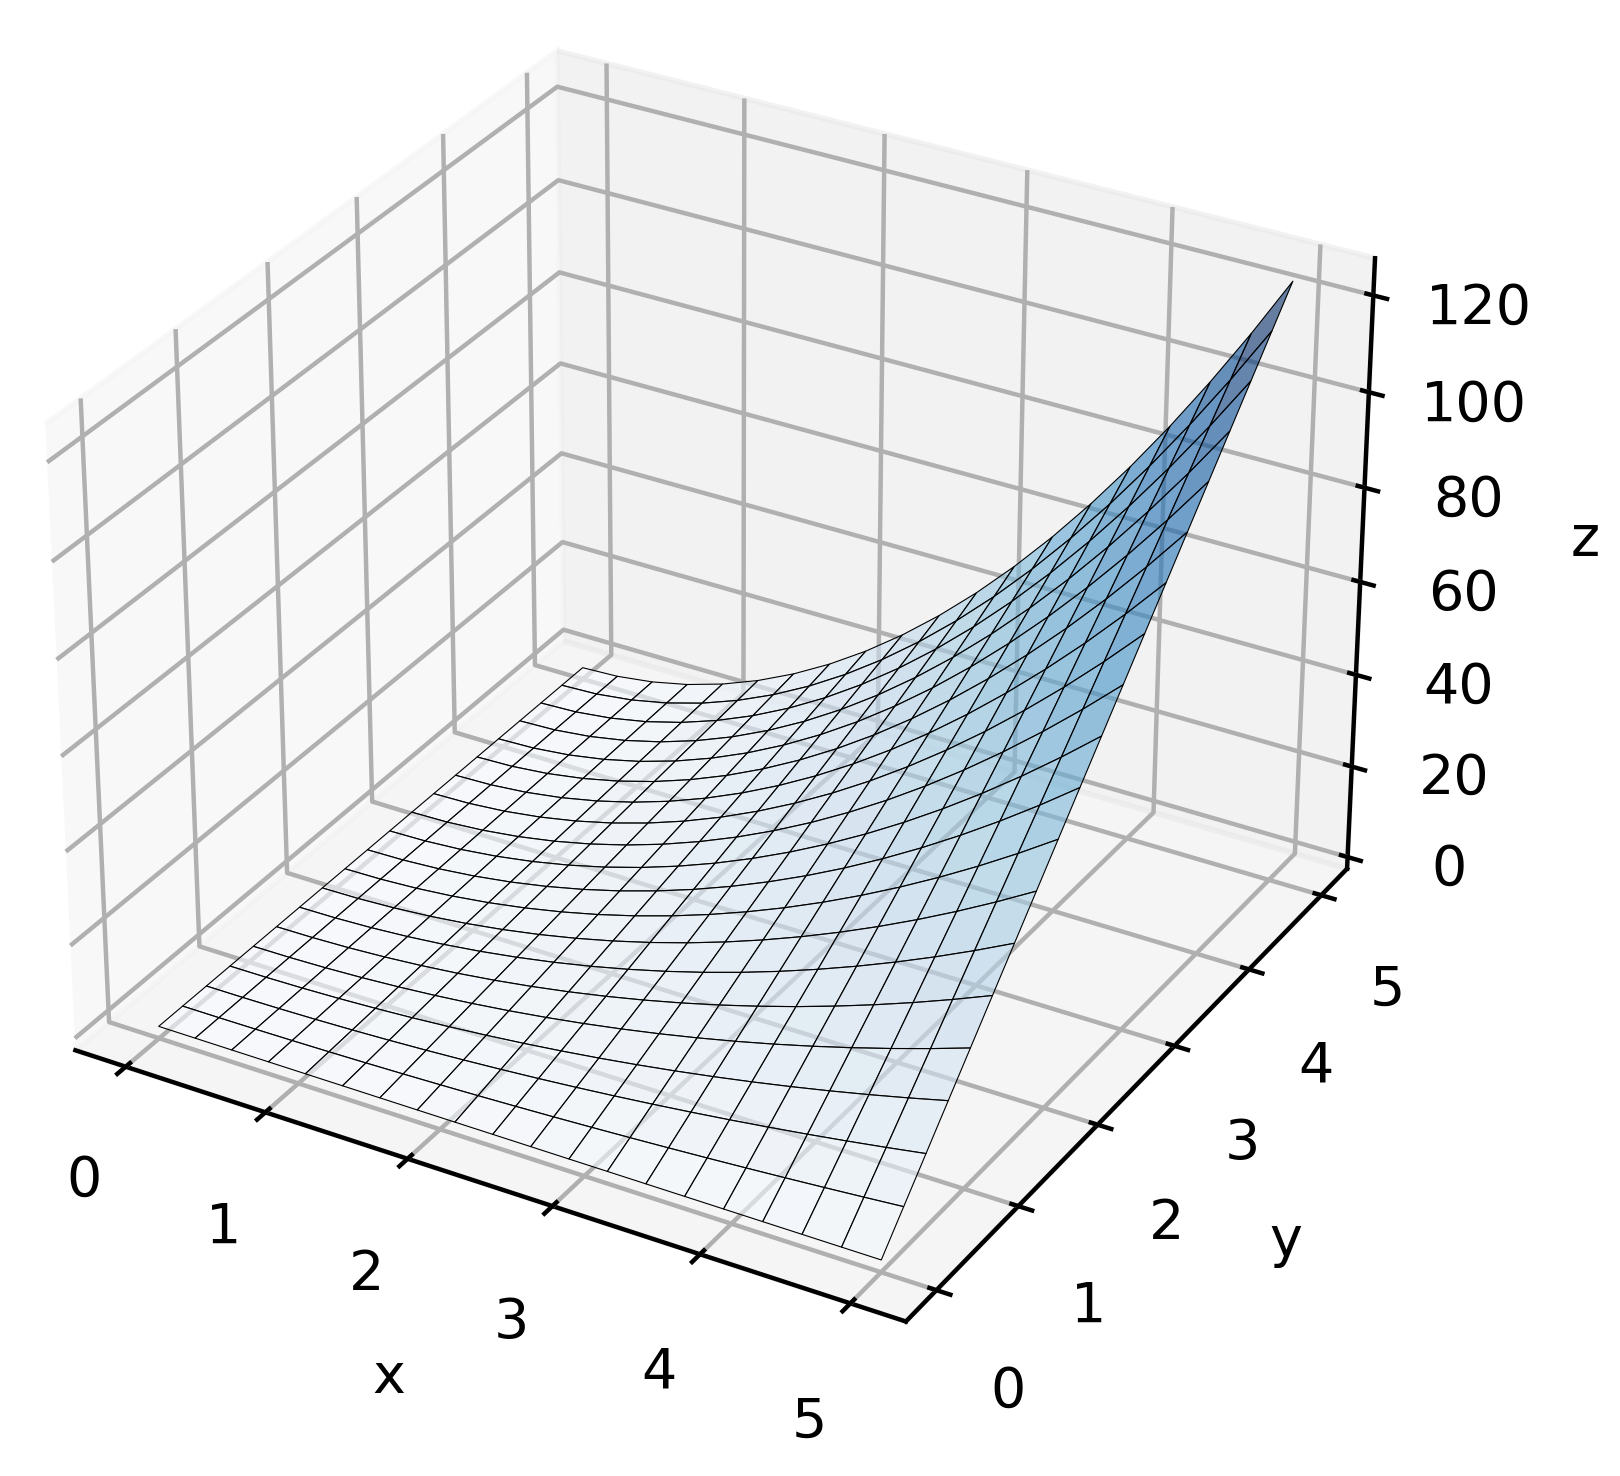
\includegraphics[scale=0.4]{figuras/der-parc2.png}
%\end{center}
%
%\end{minipage}
%
%\end{frame}
%


\begin{frame}
Se fixarmos $y=-3$ e deixarmos {\color{red}$x$} variar livremente, teremos uma função apenas da variável {\color{red}$x$}, cujo gráfico, é uma curva sobre a superfície do gráfico de de $f$.
\[f_1({\color{red}x})=f({\color{red}x},-3)=91-{\color{red}x^2}, \ -5\sqrt{2}\leq {\color{red}x}\leq 5\sqrt{2} \]

	
\begin{center}
	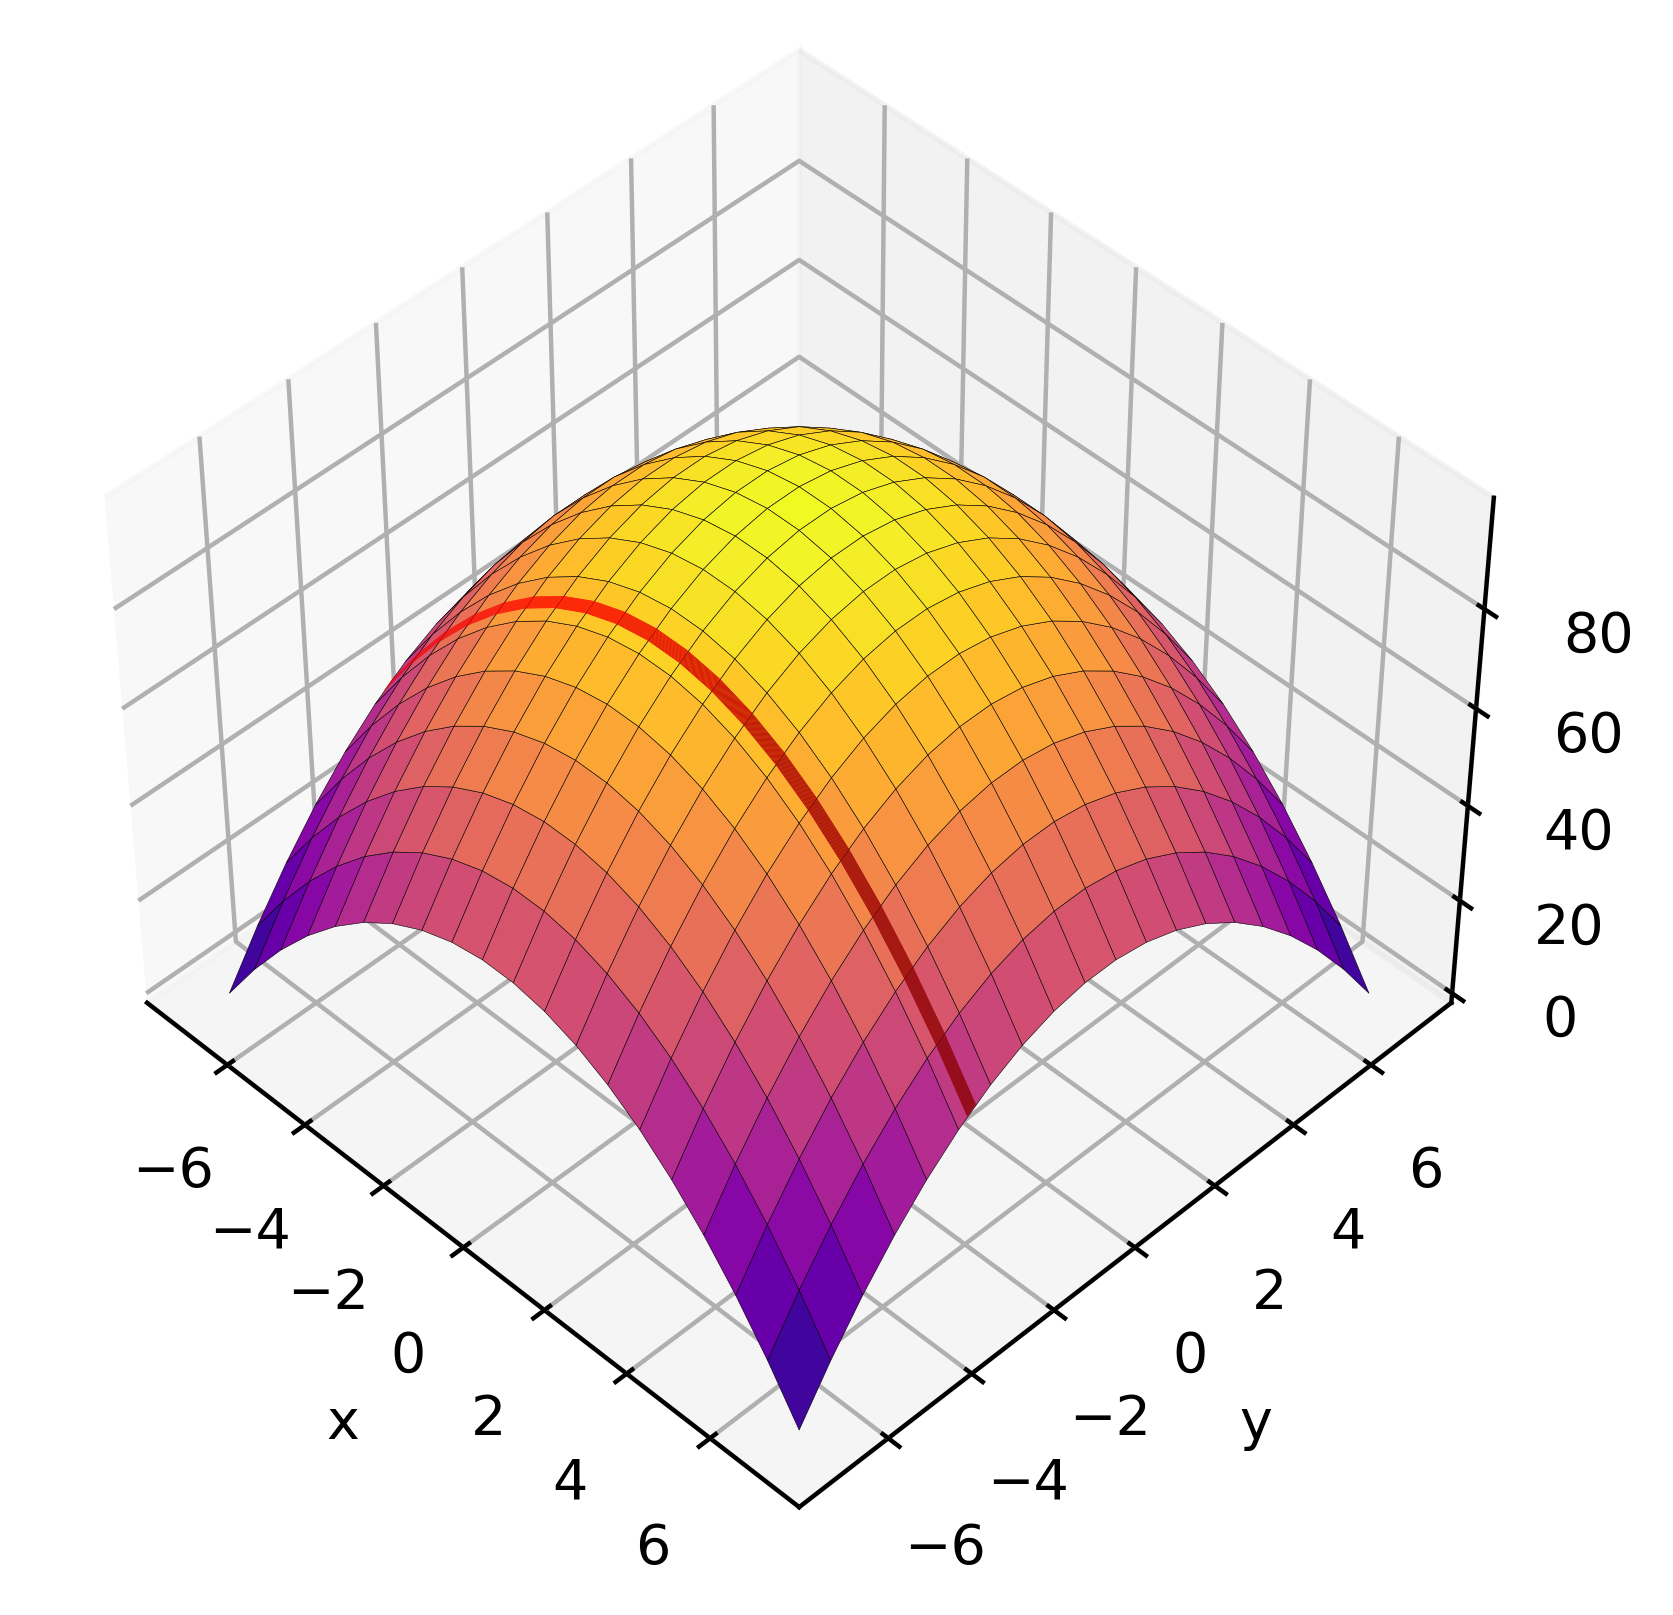
\includegraphics[scale=0.6]{figuras/der-parc2-2.png}
\end{center}
\end{frame}

\begin{frame}
	Analogamente, se fixarmos $x=2$ e deixarmos {\color{blue}$y$} variar livremente, teremos uma função apenas da variável {\color{blue}$y$}, cujo gráfico, é uma curva sobre a superfície do gráfico de de $f$.
	\[f_2({\color{blue}y})=f(2,{\color{blue}y})=96-{\color{blue}y^2}, \ -5\sqrt{2}\leq {\color{blue}y}\leq 5\sqrt{2} \]
	
	
	\begin{center}
		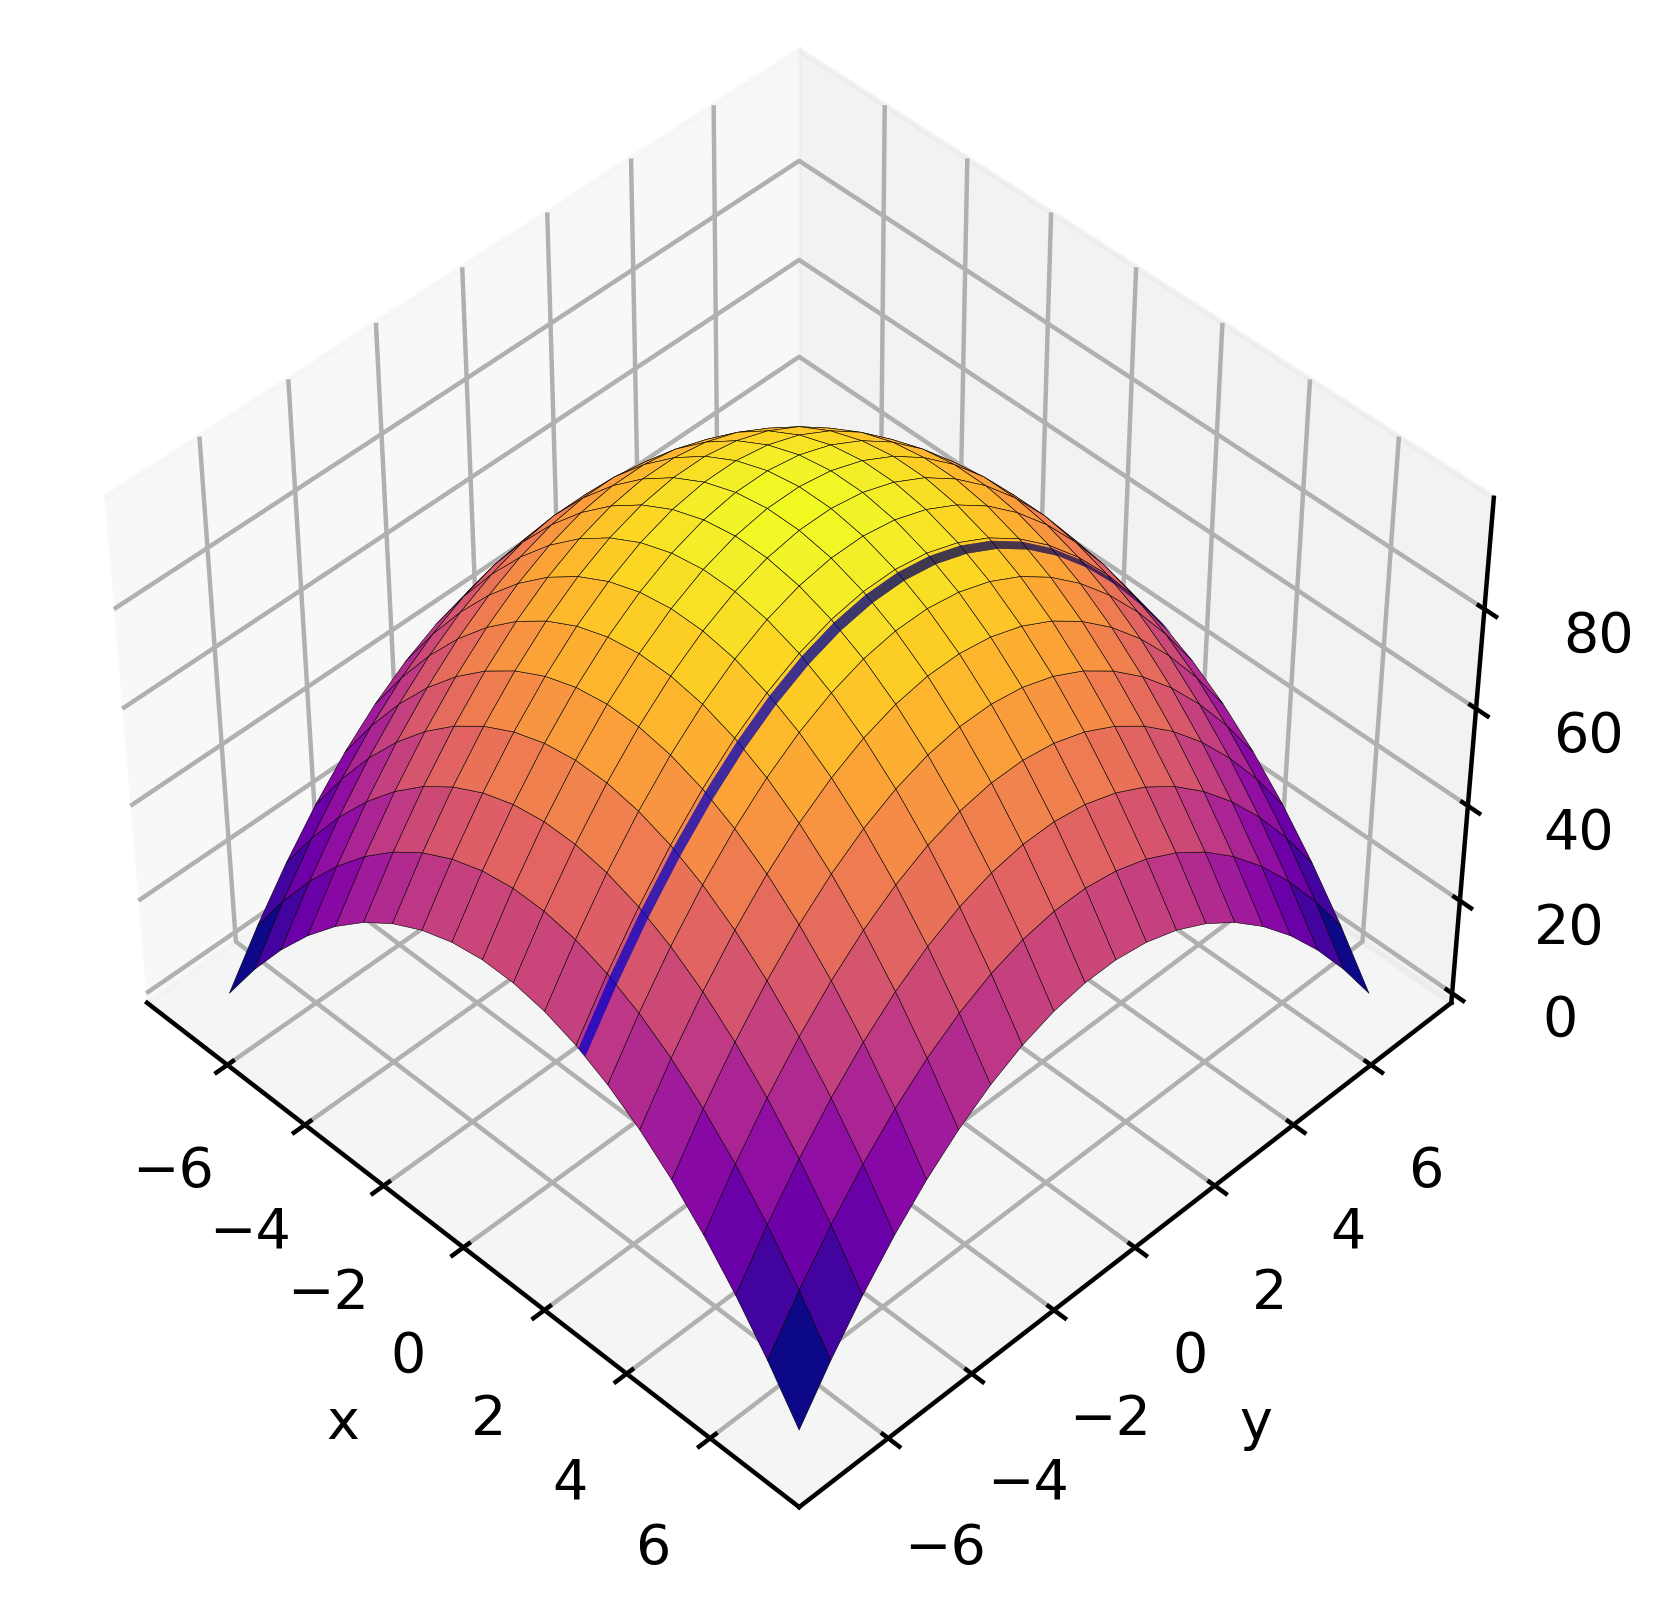
\includegraphics[scale=0.6]{figuras/der-parc2y-2.png}
	\end{center}
\end{frame}

\begin{frame}
	Em resumo, temos
	\[f_1({\color{red}x})=f({\color{red}x},-3)=91-{\color{red}x^2}, \ -5\sqrt{2}\leq {\color{red}x}\leq 5\sqrt{2} \]
	
	\[f_2({\color{blue}y})=f(2,{\color{blue}y})=96-{\color{blue}y^2}, \ -5\sqrt{2}\leq {\color{blue}y}\leq 5\sqrt{2} \]
	
	
	\begin{center}
		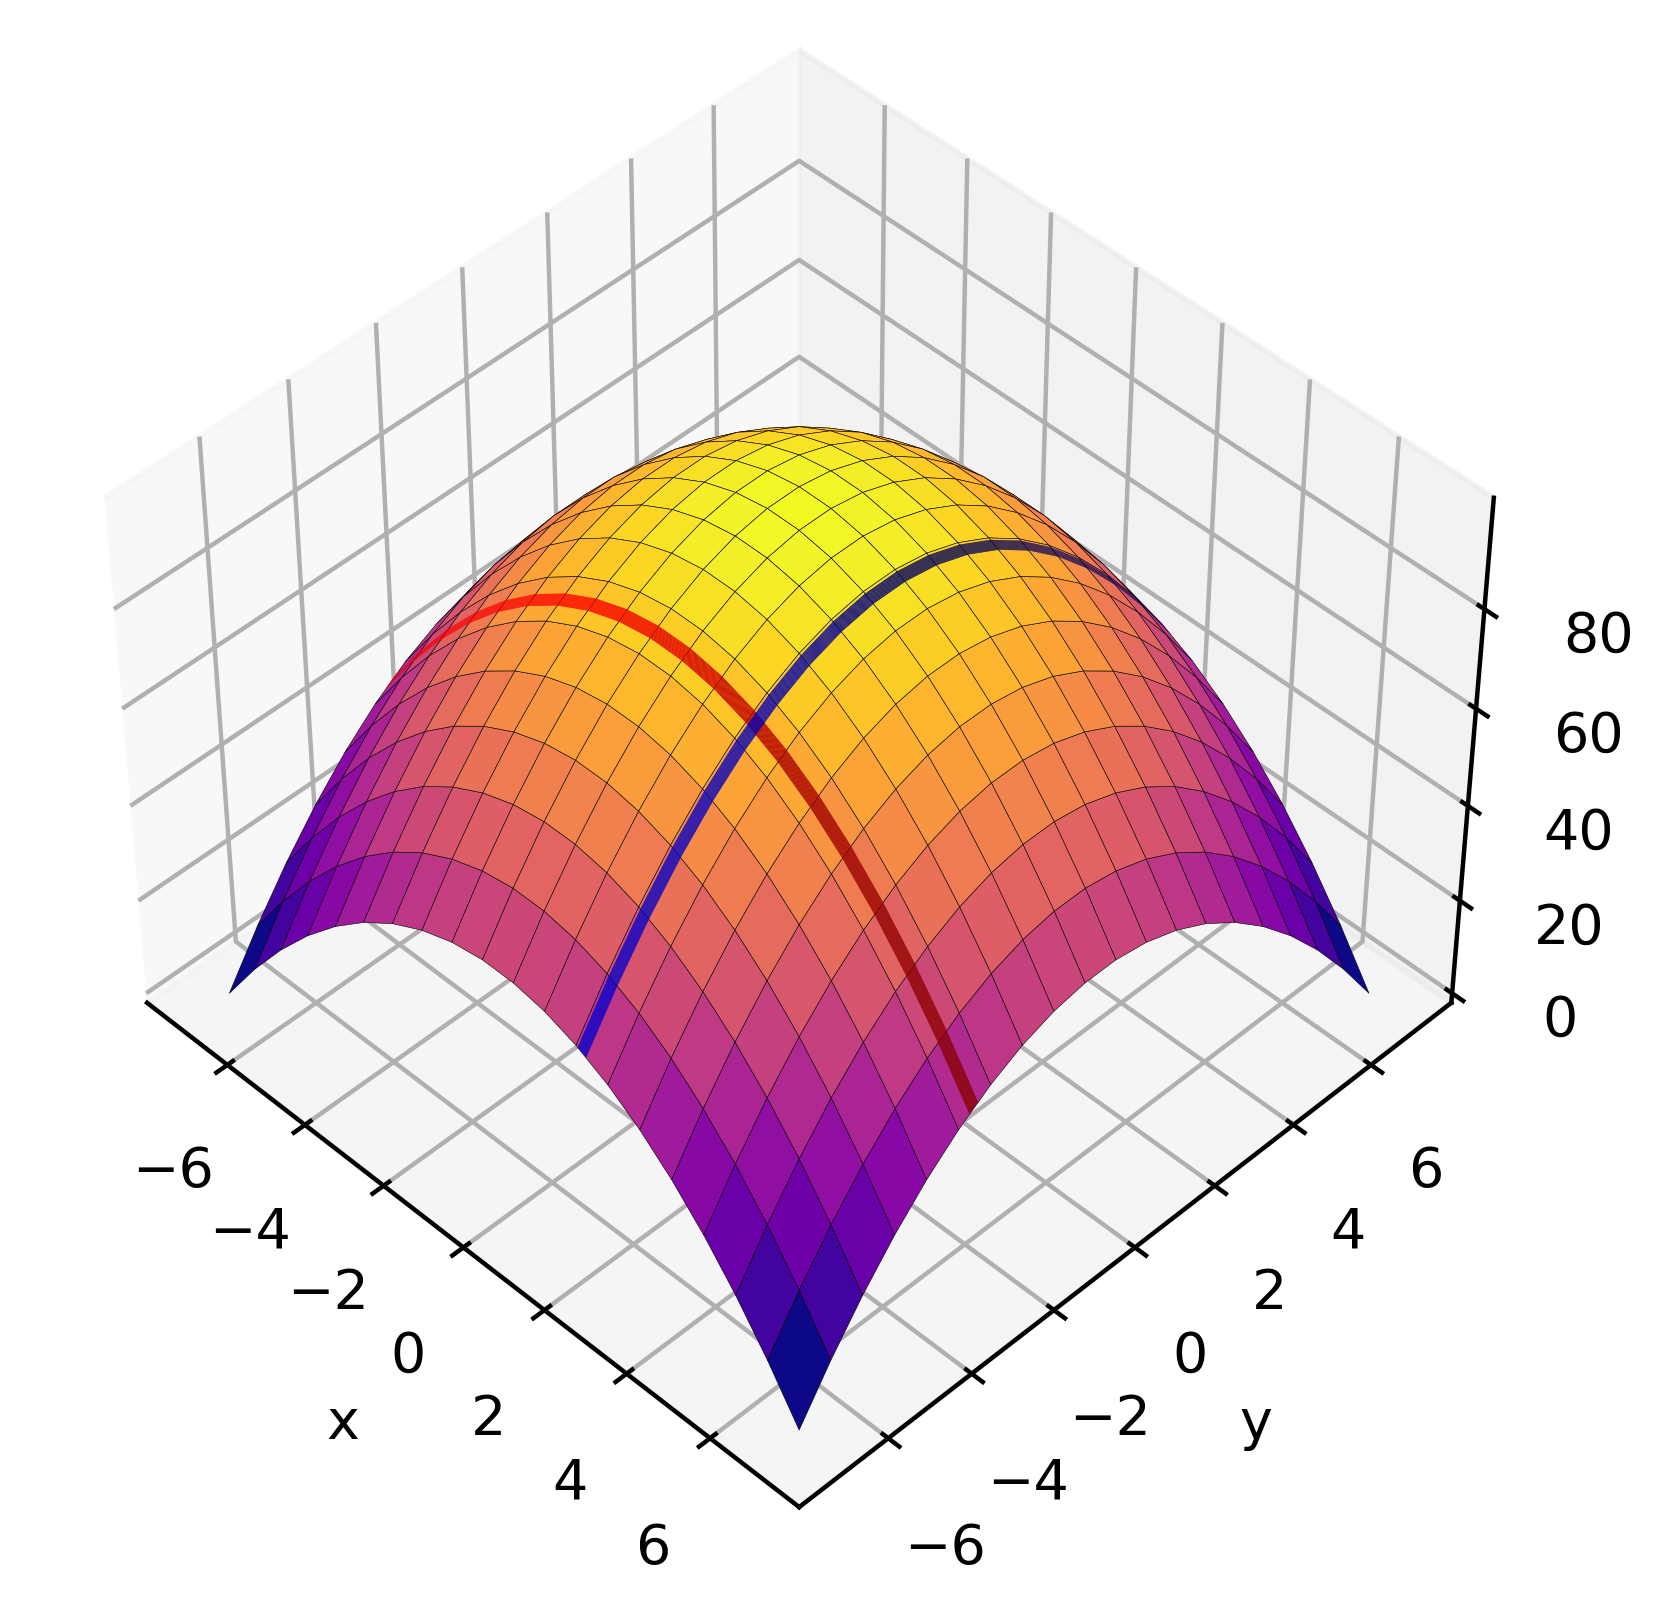
\includegraphics[scale=0.6]{figuras/der-parc2xy-2.png}
	\end{center}
\end{frame}

\begin{frame}
	É fácil ver que $f_1'({\color{red}x})=-2{\color{red}x}$. Assim, por exemplo, $f_1'(2)=-4$.
	\medskip 
	
	 Isso nos diz que a {\color{red}taxa de variação da temperatura}, no ponto $P=(2,-3)$, é de $-4^\circ C/m$ na {\color{blue}direção positiva do eixo $x$}.
	\medskip
	
	Em outras palavras, se caminharmos sobre a placa, a partir do ponto $P=(2,-3)$, {\color{blue}direção positiva do eixo $x$}, {\color{red}a temperatura vai cair a uma taxa de $-4^\circ C/m$.}
	
\begin{center}
	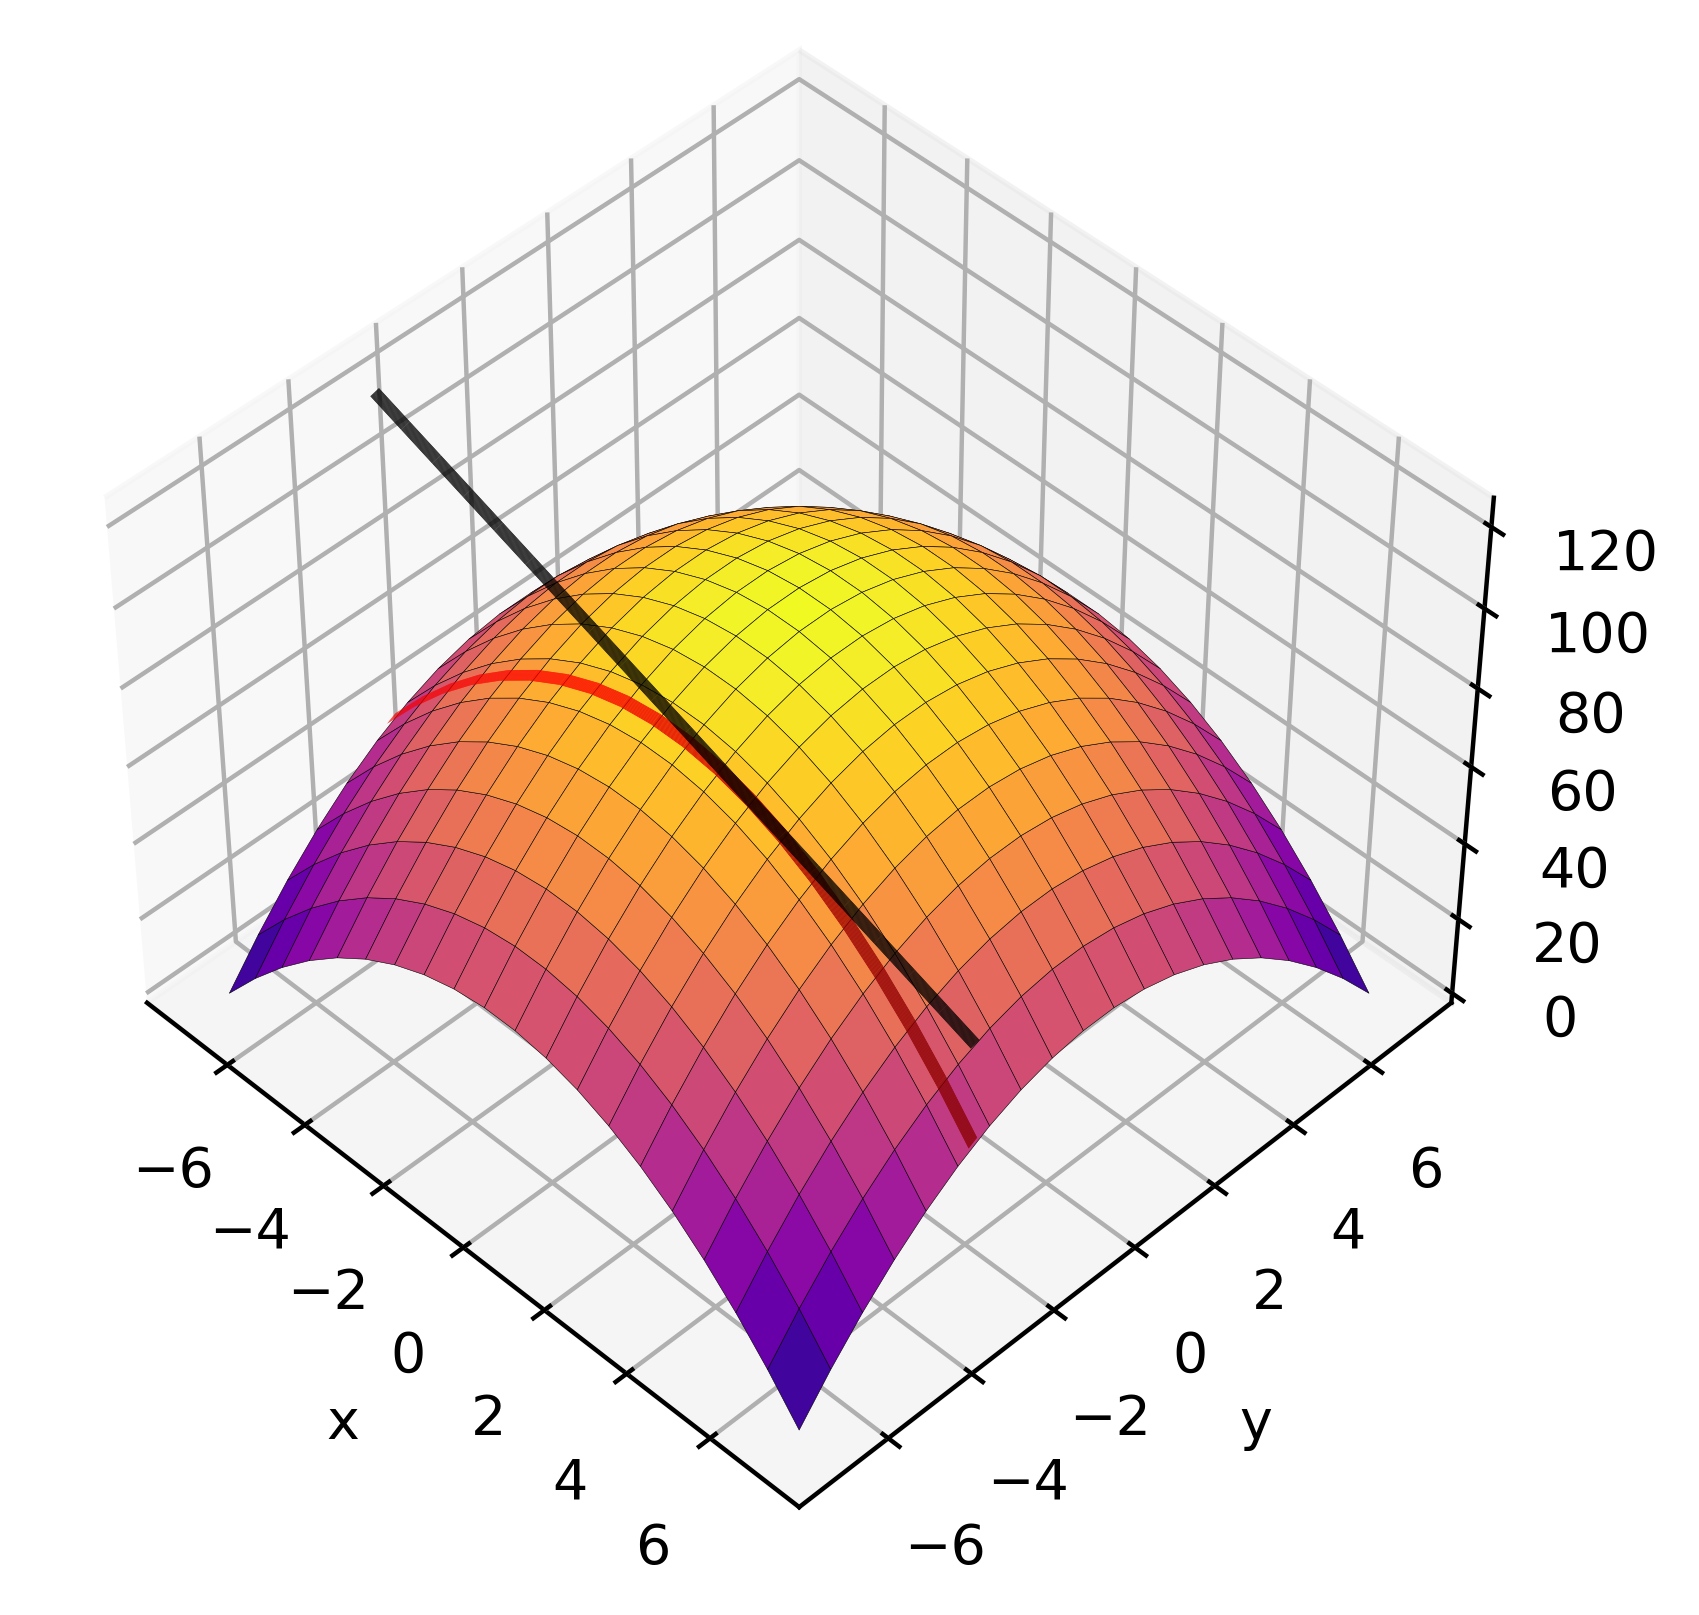
\includegraphics[scale=0.55]{figuras/der-parc2-3.png}
\end{center}
\end{frame}





\begin{frame}[label=der-parciais]
Sabemos que a derivada de $f_1$ em um ponto {\color{red} $a$} é dada por:
\[f_1'({\color{red}a})=\lim\limits_{h\to0}\frac{f_1({\color{red}a}+h)-f_1({\color{red}a})}{h}=\lim\limits_{h\to0}\frac{f({\color{red}a}+h,-3)-f({\color{red}a},2)}{h}.\]
\end{frame}


\begin{frame}[label=der-parciais]
	Sabemos que a derivada de $g$ em um ponto {\color{red} $a$} é dada por:
	\[f_1'({\color{red}a})=\lim\limits_{h\to0}\frac{f_1({\color{red}a}+h)-f_1({\color{red}a})}{h}=\lim\limits_{h\to0}\frac{f({\color{red}a}+h,-3)-f({\color{red}a},2)}{h}.\]
	De modo geral, se fixarmos um ponto genérico $y=b$, fazendo $f_1({\color{red}x})=f({\color{red}x},b)$, teremos:
	\[f_1'({\color{red}a})=\lim\limits_{h\to0}\frac{f_1({\color{red}a}+h)-f_1({\color{red}a})}{h}=\lim\limits_{h\to0}\frac{f({\color{red}a}+h,b)-f({\color{red}a},b)}{h}.\]
	Analogamente, se fixarmos um ponto genérico $x=a$, fazendo $f_2({\color{blue}y})=f(a,{\color{blue}y})$, teremos:
	\[f_2'({\color{blue}b})=\lim\limits_{h\to0}\frac{f_2({\color{blue}b}+h)-f_2({\color{blue}b})}{h}=\lim\limits_{h\to0}\frac{f(a,{\color{blue}b}+h)-f(a,{\color{blue}b})}{h}.\]
\end{frame}

\subsection*{Definição}
\begin{frame}[label=der-parciais]
%	\begin{scriptsize}
		\frametitle{}
		\uncover<1->{\begin{defin} Sejam $f:U\subset\R^2\to \R$ uma função e $(a,b)\in U$. A \dt{derivada parcial de $f$ em relação a $x$} no ponto $(a,b)$ é dada por
				$$\dx{f}(a,b)=\lim_{h\to 0}\frac{f(a+h,b)-f(a,b)}{h},$$
				quando este limite existe. Analogamente, A \dt{derivada parcial de $f$ em relação a y} no ponto $(a,b)$ é dada por
				$$\dy{f}(a,b)=\lim_{h\to 0}\frac{f(a,b+h)-f(a,b)}{h},$$
				quando este limite existe. 
		\end{defin}}
		
\begin{exe}
Se $f(x,y)=x^3+x^2y^3-2y^2$, determine $f_x(2,1)$ e $f_y(2,1)$.
\end{exe}
%	\end{scriptsize}
\end{frame}


\begin{frame}[label=der-parciais]
	\frametitle{ }
	Analogamente se $f:U\subset\R^3\to \R$ uma função definida em um aberto $U$ contendo $(x_0,y_0,z_0)$. As derivadas parcial de $f$ em relação a $x$, $y$ e $z$  no ponto $(x_0,y_0,z_0)$ são dadas pelos limites
\[\dx{f}(x_0,y_0,z_0)=\lim_{h\to 0}\frac{f(x_0+h,y_0,z_0)-f(x_0,y_0,z_0)}{h},\]
\[\dy{f}(x_0,y_0,z_0)=\lim_{h\to 0}\frac{f(x_0,y_0+h,z_0)-f(x_0,y_0,z_0)}{h},\]
\[\dz{f}(x_0,y_0,z_0)=\lim_{h\to 0}\frac{f(x_0,y_0,z_0+h)-f(x_0,y_0,z_0)}{h},\]
	quando estes limites existem. 
	
\begin{exe}
Se $f(x,y,z)=e^{xy}\log(z)$, determine as derivadas parciais.
\end{exe}
	
\end{frame}


\begin{frame}[label=der-parciais]
\begin{casa}
\begin{enumerate}
\item Se $f(x,y)=\sin\left(\frac{x}{1+y}\right)$, calcule $f_x$ e $f_y$.

\item Se $f(x,y,z)=x\sin(y-z)$, determine as derivadas parciais.
\end{enumerate}
\end{casa}
\end{frame}



\subsection*{Derivadas de Ordem Superior}
\begin{frame}[label=der-parciais]
	\frametitle{Derivadas de Ordem Superior }
%	\begin{scriptsize}
		
		\uncover<1->{ Se $z=f(x,y)$ é uma função, então  $\dx{f}$ e $\dy{f}$ também são funções de duas variáveis e portanto  podemos definir quatro novas funções que são chamadas de \dt{derivadas parciais de segunda ordem de f}, a saber:
			\begin{multicols}{2}
				$\dps f_{xx}=\frac{\partial^2f}{\partial x^2}=\dx{}\left(\dx{f}\right)$
				\bigskip
				
				$\dps f_{xy}=\frac{\partial^2f}{\partial y\partial x}=\dy{ }\left(\dx{f}\right)$
				\bigskip
				
				
				$\dps f_{yx}=\frac{\partial^2f}{\partial x\partial y}=\dx{}\left(\dy{f}\right)$
				\bigskip
				
				$\dps f_{yy}=\frac{\partial^2f}{\partial y^2}=\dy{}\left(\dy{f}\right)$
				\bigskip
		\end{multicols}}
		
		\uncover<1->{\begin{exe} Calcule todas as derivadas parciais de segunda ordem da função $f(x,y)=x^3+x^2y^3-2y^2$.
		\end{exe}}
		
		
%	\end{scriptsize}
\end{frame}




\begin{frame}[label=der-parciais]
	\frametitle{ }
	
\begin{teo} Se $z=f(x,y)$ é de classe $C^2$, então suas derivadas mistas são iguais, isto é, 
				$$\frac{\partial^2 f}{\partial x\partial y}=\frac{\partial^2 f}{\partial y\partial x}.$$
			\end{teo} 
			
%			\begin{exe} Calcule as derivadas mistas de $f$ no ponto $(0,0)$
%				$$f(x,y)=\left\{\begin{array}{ll}
%					\frac{xy^3}{x^2+y^2},& (x,y)\neq(0,0)\\
%					0, & (x,y)=(0,0)
%				\end{array}\right.$$
%		\end{exe}}
		
\end{frame}

\subsection*{EDPs}
\begin{frame}[label=der-parciais]{Equações Diferenciais Parciais - EDP}
As derivadas parciais ocorrem em {\color{blue}Equações Diferenciais Parciais} que exprimem certas leis físicas. Por exemplo, a EDP
\[u_{xx}+u_{yy}=0,\]
é chamada de {\color{blue} Equação de Laplace}. As soluções dessa equação são chamadas de {\color{blue} funções harmônicas}e são muito importantes no estudo de condução de calor, escoamento de fluidos e potencial elétrico.

\begin{exe}
Mostre que a função $u(x,y)=e^x\sin(y)$ é uma solução da equação de Laplace.
\end{exe}
\end{frame}

\begin{frame}[label=der-parciais]{Equação da Onda}
A {\color{blue}Equação da Onda}
\[u_{tt}=a^2u_{xx}\]
descreve o movimento de uma onda. Por exemplo, se $u(x,t)$ representa o deslocamento da corda vibrante de um violão no instante $t$ e à distância $x$ de uma das extremidades da corda, então $u(x,t)$ satisfaz a equação da onda. A constante $a$ depende da densidade da corda  e da tensão aplicada a nela.

\begin{exe}
Verifique que $u(x,t)=\sin(x-at)$ satisfaz a equação da onda.
\end{exe}
\end{frame}



\begin{frame}[label=der-parciais]
\begin{casa}
\begin{enumerate}
\item Calcule todas as derivadas parciais de segunda ordem da função $f(x,y)=xy-e^x\cos y$.
\item  Calcule $f_{xxyz}$ se $f(x,y,z)=\sin(3x+yz)$.
%
%
% Calcule $f_{zx}$ e $f_{xz}$ da função $f(x,y,z)=\log(x^2+y^2+z^2)$.
\end{enumerate}
\end{casa}
\end{frame}

%
%
%\begin{frame}[label=der-parciais]
%	\frametitle{ }
%	
%	\uncover<1->{\begin{exe}
%			%\begin{multicols}{3}
%			\begin{enumerate}
%				\item $f(x,y)=x^2+y$
%				\item $f(x,y,z)=xe^{x+y+z}$
%				\item $f(x,y)=\left\{\begin{array}{ll}
%					\frac{xy}{x^2+y^2},& (x,y)\neq (0,0)\\
%					0,& (x,y)= (0,0)\\
%				\end{array}\right.$
%			\end{enumerate}
%			%\end{multicols}
%	\end{exe}}
%	
%	\uncover<2->{Sabemos que se $f$ é uma função de uma variável derivável em $x_0$, então $f$ é contínua é contínua em $x_0$.}
%	\bigskip
%	
%	\uncover<3->{\textcolor{red}{Pergunta: Se $f$ é uma função de duas variáveis com derivadas parciais em $(x_0,y_0)$, então $f$ é contínua?! }}
%	
%\end{frame}

\subsection*{Aproximação Linear}

\begin{frame}[label=der-parciais]
	\frametitle{Aproximação Linear em uma variável}
%	\begin{scriptsize}
Em funções de uma variável sabemos que se {\color{blue}$f(x)$ é derivável em $x_0$}, sabemos que a reta tangente ao gráfico de $f$ no ponto $(x_0,f(x_0))$ é dada por
			\[L(x)=f(x_0)+f'(x_0)(x-x_0).\]
			Assim, para pequenos acréscimos $\Delta x$ na quantidade $x_0$, o valor de $f(x_0+\Delta x)$ é aproximadamente $L=f(x_0)+f'(x_0)\Delta x$, com erro
			\[E(\Delta x)=f(x_0+\Delta x)-f(x_0)-f'(x_0)\Delta x,\]
			onde {\color{red}$\dps\lim_{\Delta x\to 0}\frac{E(\Delta x)}{\Delta x}=0.$} Em outras palavras, o erro $E$ é menor que o erro $\Delta x$, para valores pequenos de $\Delta x$.
			
			
			Neste caso dizemos que $f$ é {\color{blue} diferenciável} e  que 
\[{\color{red}L(x)=f(x_0)+f'(x_0)(x-x_0)}\]
é uma {\color{red} aproximação linear} de $f$ no ponto $x_0$.
		
%		\uncover<1->{Com isso, para ver que $f$ é contínua em $x_0$ basta calcular o seguinte limite
%			$$\lim_{h\to 0}f(x_0+h)=\lim_{h\to 0}(f'(x_0)h+f(x_0)+E(h))=f(x_0)$$}
		
%	\end{scriptsize}
\end{frame}


\begin{frame}[label=der-parciais]
	\frametitle{Plano Tangente }
%	\begin{scriptsize}
		
		\uncover<1->{Como podemo obter o plano tangente ao gráfio da função  {\color{blue}$f(x,y)=9-x^2-y^2$} no ponto $P=(1,2,4)$?  }
		\bigskip 
		
Fixando  $y=2$ e fazendo $x$ variar, temos a curva sobre o gráfico passando por $P$
\[{\color{red}\alpha(x)=(x,2,5-x^2),\ x\in \R.}\]
cujo  o vetor tangente em $P$ é
\[{\color{red}u=\alpha'(1)=(1,0,-2).}\] 
Analogamente obtemos que outro vetor tangente ao gráfico no ponto $P$ é
\[{\color{cyan}v=(0,1,-4)}.\] 
Como {\color{cyan}$u$} e {\color{red}$v$} são LI, sabemos que o produto vetorial é um vetor normal ao plano, daí, obtemos que a equação do plano tangente é 
			\[2x+2y+z-10=0.\]
	
		
%	\end{scriptsize}
\end{frame}


\begin{frame}[label=der-parciais]
No caso geral, se $z=f(x,y)$, então o \dt{plano tangente} no ponto $P=(x_0,y_0,z_0)$ é dado pela equação
\begin{equation}\label{plano_tang}
{\color{blue}z=f(x_0,y_0)+\dx{f}(x_0,y_0)(x-x_0)+\dy{f}(x_0,y_0)(y-y_0).}
\end{equation}
O plano tangente é a {\color{red} melhor aproximação linear} da função {$z=f(x,y)$}	nas proximidades do ponto $P=(x_0,y_0,z_0)$ e a função 
\[{\color{red}L(x,y)=f(x_0,y_0)+\dx{f}(x_0,y_0)(x-x_0)+\dy{f}(x_0,y_0)(y-y_0)}\]
é denominada {\color{red}linearização} de $f$ no ponto $(x_0,y_0)$. 
\bigskip

\begin{alertblock}{ }
Diferentemente do caso unidimensional, para que essa aproximação seja boa, {\color{red}não é suficiente} que apenas existam as derivadas parciais. Para isso, precisamos definir uma noção de diferenciabilidade análoga.
\end{alertblock}
			
\end{frame}







\subsection*{Diferenciabilidade}
\begin{frame}[label=der-parciais]
	\frametitle{ }
%	\begin{scriptsize}
		
		\uncover<1->{\begin{defin}
				Uma $f:U\to \R$, definida no aberto $U\subset \R^2$, é dita \dt{diferenciável
				 em $(x_0,y_0)\in U$} quando existem $\dx{f}(x_0,y_0)$, $\dy{f}(x_0,y_0)$ tais que a função erro definida por 
\begin{multline*}
 E(\Delta x,\Delta y)=\\
 f(x_0+\Delta x,y_0+\Delta y)-f(x_0,y_0)-\dx{f}(x_0,y_0)\Delta x-\dy{f}(x_0,y_0) \Delta y,
\end{multline*}
satisfaz, $\displaystyle\lim_{(\Delta x,\Delta y)\to(0,0)}\frac{E(\Delta x,\Delta y)}{\|(\Delta x,\Delta y)\|}=0$
		\end{defin}}
		
\begin{alertblock}{ }
Esta definição diz que uma função diferenciável é aquela para a qual a aproximação linear é uma boa aproximação quando $(x,y)$ está próximo de $(x_0,y_0)$.
\end{alertblock}
	
\end{frame}

\begin{frame}[label=der-parciais]
\begin{exe}
Mostre que $f(x,y)=2x^2+y^2$ é diferenciável em $(1,1)$ e determine a aproximação linear.
\end{exe}

\begin{exe}
Mostre que a função $f(x,y)=x^{1/3}y^{1/3}$, possui derivadas parciais no ponto $(0,0)$ mas não é diferenciável, isto é, a equação do que seria o plano tangente existe, mas não fornece uma boa aproximação.
\end{exe}
\end{frame}


%
%\begin{frame}
%		\uncover<1->{\begin{teo} 
%				Se $f$ é diferenciável em $(x_0,y_0)$, então $f$ é contínua em $(x_0,y_0)$.
%		\end{teo}}
%		
%		\uncover<1->{Com essa definição podemos precisar o que é uma função ser ``suave''. Assim, podemos dizer que uma função é \dt{suave} quando existe o plano tangente ao gráfico da função, ou seja, quando $f$ é diferenciável. Note que  }
%%	\end{scriptsize}
%\end{frame}


\begin{frame}[label=der-parciais]
%	\frametitle{ }
%	\uncover<1->{\begin{exe}
%			\begin{enumerate}
%				\item Mostre que $f(x,y)=x^2+y^2$ é diferenciável em $\R^2$.
%				\item $f(x,y)=\left\{\begin{array}{ll}
%					\frac{x^2y}{x^4+y^2},&(x,y)\neq(0,0)\\
%					0, &(x,y)=(0,0)\\
%				\end{array}\right.$ é diferenciável em $(0,0)$?
%			\end{enumerate}
%	\end{exe}}
	
	\uncover<1->{\begin{defin} Uma função $f:U\to \R$, definida em um aberto $U\subset\R^2$, é dita de {\color{blue}classe $C^1$ em $U$} quando possui derivadas parciais contínuas em $U$. 
	\end{defin}}
	
	\uncover<1->{\begin{teo}\label{teo_dif} Se $f:U\to \R$ é de classe $C^1$ em $U$, então $f$ é diferenciável em $U$.
	\end{teo}}
	
	\begin{exe}
	Mostre que $f(x, y) = xe^{xy}$ é diferenciável em $(1, 0)$ e encontre sua linearização ali. Em seguida, use a linearização para aproximar $f( 1.1,-0.1)$.
	\end{exe}
\end{frame}


\subsection*{Diferenciais}
\begin{frame}[label=der-parciais]{Diferenciais}
Para uma função diferencial de uma única variável, $y = f(x)$, definimos a diferencial $dx$ como uma variável independente, ou seja, $dx$ pode valer qualquer número real. {\color{blue}A diferencial de $y$} é definida como
\[dy=f'(x) dx\]
\begin{center}
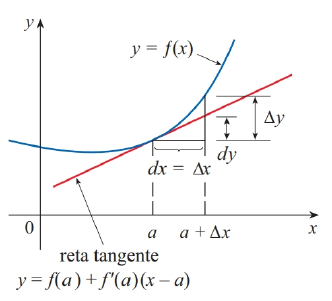
\includegraphics[scale=0.5]{figuras/diferenciais1.png}
\end{center}
\end{frame}

\begin{frame}[label=der-parciais]
Para uma função de duas variáveis, $z = f (x, y )$, definimos as diferenciais $dx$ e $dy$ como
variáveis independentes. Então, a {\color{blue}diferencial $dz$}, também chamada de {\color{blue} diferenciação total}, é definida por
\[dz
=\frac{\partial z}{\partial x}dx+\frac{\partial z}{\partial y}dy
=f_x(x,y)dx+f_y(x,y)dy\]
\begin{center}
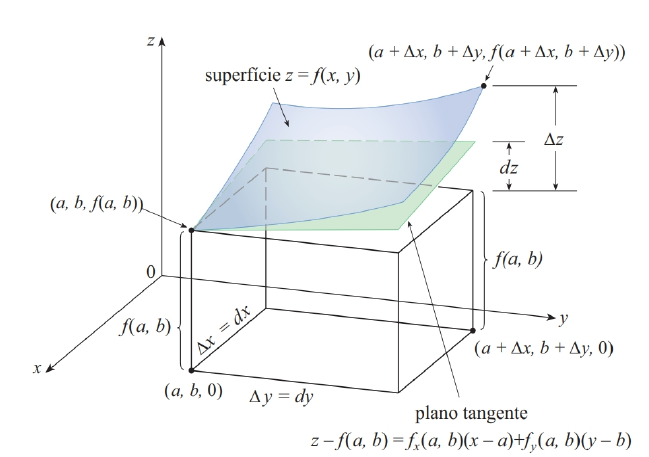
\includegraphics[scale=0.4]{figuras/diferenciais2.png}
\end{center}

\end{frame}

\begin{frame}[label=der-parciais]
\begin{exe}
Foram feitas medidas do raio da base e da altura de um cone circular reto e obtivemos 10 cm e 25 cm, respectivamente, com possível erro nessas medidas de, no máximo, $\varepsilon$ cm.
\begin{enumerate}
\item Use diferenciais para estimar o erro máximo cometido no cálculo do volume do
cone.

\item Se o raio e a altura forem medidos com erro máximo de 0.1 cm, qual será o erro máximo estimado para o volume? Estime o erro relativo.
\end{enumerate}
\end{exe}
\end{frame}

\begin{frame}[label=der-parciais]{Funções de três Variáveis}
Aproximações lineares, diferenciabilidade e diferenciais podem ser definidas de maneira análoga para as funções de mais que duas variáveis. 
\medskip


\begin{block}{Diferenciabilidade}
Uma função  $w=f(x,y,z)$ é {\color{blue} diferenciável em $(x_0,y_0,z_0)$} quando existem as derivadas parciais no ponto $(x_0,y_0,z_0)$ e 
\begin{multline*}
 E(\Delta x,\Delta y,\Delta z)=
 f(x_0+\Delta x,y_0+\Delta y,z_0+\Delta z)-f(x_0,y_0,z_0)\\-\dx{f}(x_0,y_0,z_0)\Delta x-\dy{f}(x_0,y_0,z_0) \Delta y-\dz{f}(x_0,y_0,z_0)\Delta z,
\end{multline*}
satisfaz, $\displaystyle\lim_{(\Delta x,\Delta y,\Delta z)\to(0,0,0)}\frac{E(\Delta x,\Delta y,\Delta z)}{\|(\Delta x,\Delta y,\Delta z)\|}=0$
\end{block}



\end{frame}



\begin{frame}[label=der-parciais]
Se $w=f(x,y,z)$ é diferenciável em $(x_0,y_0,z_0)$, então 
\bigskip

A {\color{blue}linearização} de $f$ no ponto $(x_0,y_0,z_0)$. 
{\color{blue}\begin{multline*}
L(x,y,z)=f(x_0,y_0,z_0)+\dx{f}(x_0,y_0,z_0)(x-x_0)\\+\dy{f}(x_0,y_0,z_0)(y-y_0)+\dz{f}(x_0,y_0,z_0)(z-z_0)
\end{multline*}}

A {\color{blue}diferencial $dw$}  é definida por
{\color{blue}
\[dw=\dx{w}dx+\dy{w}dy+\dz{w}dz.\]}



\end{frame}


\begin{frame}[label=der-parciais]
	\frametitle{ }
	\uncover<1->{\begin{casa}
			\begin{enumerate}
				\item Para quais valores de $(x,y)$,  $f(x,y)=\log(x^2+y^2)$ é diferenciável é diferenciável? Justifique.
				\item Mostre que $f(x,y)=\left\{\begin{array}{ll}
					\frac{xy}{x^2+y^2},& (x,y)\neq (0,0)\\
					0,& (x,y)= (0,0)\\
				\end{array}\right.$ não é diferenciável em $(0,0)$ mas possui derivadas parciais em $\R^2$.
			\end{enumerate}
	\end{casa} }
	
%	\uncover<2->{\begin{obs} A recíproca do Teorema \ref{teo_dif} é falsa, ou seja, existem funções diferenciáveis que não são de classe $C^1$. Um exemplo é a função
%			$$f(x,y)=\left\{\begin{array}{ll}
%				(x^2+y^2)\sen\left(\frac{1}{x^2+y^2}\right), &  (x,y)\neq (0,0)\\
%				0, & (x,y)=(0,0)\\
%			\end{array} \right.$$ 
%	\end{obs}}
\end{frame}


%\begin{frame}
%	\frametitle{Aplicação Função de Cobb-Douglas}
%	\begin{scriptsize}
%		
%		\uncover<1->{ Considere que uma empresa cuja produção possa ser modelada pela
%			seguinte função de Cobb-Douglas: $f(x,y)=10x^{0,4}y^{0,6}$, onde $f(x,y)$ é o valor da produção (medido em milhares de reais), $x$ é o investimento feito em infra-estrutura e maquinário e $y$ é o investimento feito em mão-de-obra (ambos medidos em milhares de reais). A característica dessa função é que a produção de sua empresa depende mais de mão-de-obra do que da infra-estrutura e maquinário. No momento a empresa tem R\$ 100.000 investidos em infra-estrutura e R\$ 200.000 em mão-de-obra, portanto está produzindo o equivalente a R\$ 1.515.716. Com isso, pergunta-se:}
%		
%		\uncover<2->{\begin{enumerate}
%				\item Qual a variação da produção quando mantemos a quantidade de trabalho constante e variamos a quantidade de capital? E quanto é a variação da produção quando mantemos o capital constante?
%				
%				\item Imagine que a empresa tenha possibilidade de investir mais R\$ 10.000 em infra-estrutura ou mão-de-obra, qual será o ganho aproximado na produção em cada caso? Você como Engenheiro de Produção indicaria qual opção para a empresa?
%				
%				
%		\end{enumerate}}
%		
%		
%		
%	\end{scriptsize}
%\end{frame}


\subsection*{Regra da Cadeia e Vetor Gradiente}


\begin{frame}[label=der-parciais]
	\frametitle{Regra da Cadeia e Vetor Gradiente }
%	\begin{scriptsize}
		
		\uncover<1->{\begin{block}{Regra da Cadeia 1} Sejam $z=f(x,y)$ uma função diferenciável e $\alpha(t)=(x(t),y(t))$, $t\in I$ também  diferenciável, então a função composta $z(t)=f(\alpha(t))$ é diferenciável e				\[\frac{dz}{dt}=\dx{z}\frac{dx}{dt}+\dy{z}\frac{dy}{dt}
		\]	\end{block} 
			
		}
\begin{minipage}{0.6\textwidth}
\begin{exe}
Se $z=x^2y+3xy^4$, onde $x=\sin(2t)$ e $y=\cos(t)$, determine $\frac{dz}{dt}$ em $t=0$.
\end{exe}
\end{minipage}
\begin{minipage}{0.3\textwidth}
\begin{center}
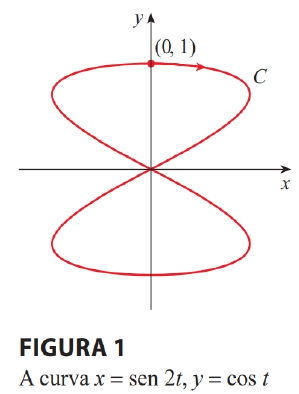
\includegraphics[scale=.4]{figuras/cadeia1.png}
\end{center}

\end{minipage}%	\end{scriptsize}
\end{frame}



%\begin{frame}
%	\frametitle{ }
%	\begin{scriptsize}
%		
%		\uncover<1->{\begin{exe}\begin{enumerate}
%					\item Sejam $z=f(x,y)=x^3y^2$, $x(t)=e^{-t}$ e $y(t)=t\sen t$. Calcule $\frac{dz}{dt}$.
%					
%					\uncover<2->{\item Certa vez, na logoa do Iriry, um grupo de estudantes de engenharia observou  que todos os dias, no mesmo horário, um pato partia de um ponto da lagoa e em 2 minutos atravessava a lagoa seguindo sempre uma mesma trajetória. 
%						\bigskip
%						
%						Determinados a entender os hábitos peculiares daquele pato, os estudantes construíram um sistema de coordenadas na lagoa, com origem no ponto de partida do pato e observaram que para cada ponto $(x,y)$ da lagoa poderiam associar uma função temperatura $T(x,y)$. Supondo que as temperaturas não variavam muito perto de um ponto da lagoa, assumiram que a função $T$ era diferenciável.  Além disso eles conseguiram descrever a trajetória do pato pela função $(x,y)=(t^2+1,3t)$ para cada instante $t$. Logo em seguida fizeram medições no lago e obtiveram que $T(5,6)=40$, $T_x(5,6)=4$, $T_y(5,6)=-2$. Com esses dados em mãos eles determinaram a taxa com que a temperatura variava em função do tempo no instante $t=2$. Qual é a taxa que eles obtiveram?}
%				\end{enumerate} 
%				
%		\end{exe} }
%		
%	\end{scriptsize}
%\end{frame}




\begin{frame}[label=der-parciais]
	\frametitle{ }
%	\begin{scriptsize}
\begin{minipage}{0.6\textwidth}
\begin{block}{Regra da Cadeia 2}
Sejam $z=f(x,y)$,  $x=x(t,s)$ e $y=y(t,s)$ são funções diferenciáveis, então
\begin{enumerate}[a]
	\item $\dps\frac{\partial z}{\partial s}={\color{red}\dx{z}}{\color{orange}\frac{\partial x}{\partial s}}+{\color{red}\dy{z}}{\color{orange}\frac{\partial y}{\partial s}}$
	\item $\dps\frac{\partial z}{\partial t}={\color{red}\dx{z}}{\color{cyan}\frac{\partial x}{\partial t}}+{\color{red}\dy{z}}{\color{cyan}\frac{\partial y}{\partial t}}$

		\end{enumerate} 
\end{block}
\end{minipage}\qquad
\begin{minipage}{0.3\textwidth}
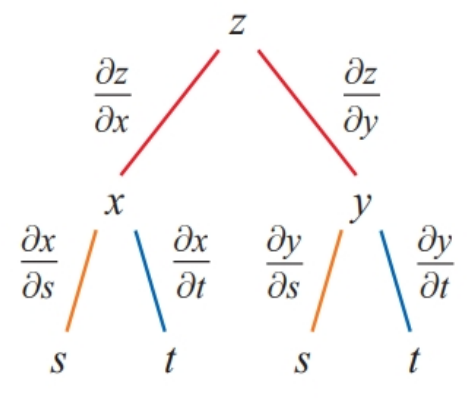
\includegraphics[scale=.3]{figuras/cadeia2.png}
\end{minipage}
\uncover<1->{\begin{exe} Calcule as derivadas parciais da função $z=e^x\sin(y)$, onde $x=st^2$ e $y=s^2t$
		\end{exe}}
		
%	\end{scriptsize}
\end{frame}



\begin{frame}[label=der-parciais]
	\frametitle{ }
%	\begin{scriptsize}
\begin{block}{Regra da Cadeia Caso Geral}
Sejam $u=u(x_1,x_2,\ldots,x_n)$ e $x_j=x_j(t_1,t_2,\ldots,t_m)$ funções diferenciáveis, então
\[\frac{\partial u}{\partial t_i}=\frac{\partial u}{\partial x_1}\frac{\partial x_1}{\partial t_i}+\frac{\partial u}{\partial x_2}\frac{\partial x_2}{\partial t_i}+\cdots +\frac{\partial u}{\partial x_n}\frac{\partial x_n}{\partial t_i}=\sum_{k=1}^{n}\frac{\partial u}{\partial x_k}\frac{\partial x_k}{\partial t_i}
\]
\end{block}

\uncover<1->{\begin{exe}
Se $u=x^4y+y^2z^3$, onde $x=rse^t$, $y=rs^2e^{-t}$ e $z=r^2s\sin(t)$, determine $\frac{\partial u}{\partial s}$ quando $r=2, s=1$ e $t=0$.
		\end{exe}}
		
%	\end{scriptsize}
\end{frame}


\begin{frame}[label=der-parciais]
\begin{casa}
\begin{enumerate}
\item Se $g(s,t)=f(s^2-t^2,t^2-s^2)$ e $f$ é diferenciável, mostre que $g$ satisfaz
\[t\frac{\partial g}{\partial s}+s\frac{\partial g}{\partial t}=0.\]

\item O raio de um cone circular reto está aumentando em uma taxa de 4.6 cm/s enquanto sua altura está descendo a uma taxa de 6.5 cm/s. Em qual taxa o volume do cone está variando quando o raio é 300 cm e altura é de 350 cm.
\end{enumerate}
\end{casa}
\end{frame}

\begin{frame}[label=der-parciais]
	\frametitle{ }
%	\begin{scriptsize}
		
		\uncover<1->{\begin{defin}Seja $f$ uma função de $n$ variáveis $x_1,\ldots,x_n$ que possui derivadas parciais no ponto $P_0=(a_1,\ldots,a_n)$. O \dt{vetor gradiente} de $f$ em $P_0$, denotado por $\nabla f(P_0)$, é o vetor
				$$\nabla f(P_0)=\left(\frac{\partial f}{\partial x_1},\ldots,\frac{\partial f}{\partial x_n}\right)$$
		\end{defin} }
		
		\uncover<1->{Usando a definição de vetor gradiente, a regra da cadeia pode ser escrita da forma
			$$\frac{dz}{dt}=\nabla f(\alpha(t))\cdot \alpha'(t).$$
			
			\begin{teo} Seja $z=f(x,y)$ uma função de classe $C^1$ definida em um aberto $U\subset \R^2$. O vetor gradiente é normal a qualquer curva de nível da função $f$ nos pontos em que não se anula.
		\end{teo}}
		
%	\end{scriptsize}
\end{frame}


\begin{frame}[label=der-parciais]
	\frametitle{ }
	
	\uncover<1->{O Teorema anterior também é válido para funções de três variáveis. Neste caso o vetor gradiente é normal à superfície de nível $F(x,y,z)=k.$ Este resultado pode ser usado para encontrar plano tangente à superfícies que não estão expressas como gráfico de função.
	
	\begin{center}
	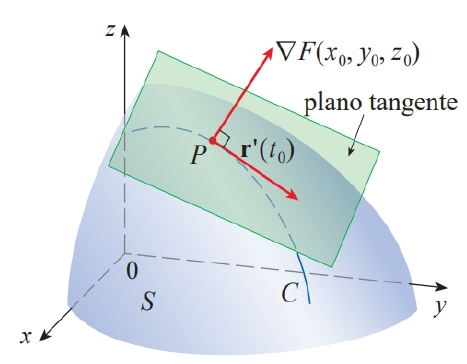
\includegraphics[scale=0.4]{figuras/plano-tang.png}
	\end{center}
		
		\begin{exe} Determine  as equações do plano tangente e da reta normal à superfície $S$ de equação $x^2+3y^2+4z^2=8$ em $(1,-1,1)$.
	\end{exe} }
	
\end{frame}

\subsection*{Derivadas Direcionais em duas variáveis}


\begin{frame}[label=der-parciais]
	\frametitle{ Derivadas Direcionais}
%	\begin{scriptsize}
		
		\uncover<1->{\begin{defin} A \dt{derivada direcional} de uma função $z=f(x,y)$ em um ponto $P_0=(x_0,y_0)$ na direção do {\color{red}vetor unitário $u=(a,b)$}  é definida por
\begin{multline*}
\frac{\partial f}{\partial {\color{red}u}}(P_0)=\lim_{ {\color{blue}h}\to 0} \frac{f(P_0+{\color{blue}h}{\color{red}u})-f(P_0)}{{\color{blue}h}}
\\=\lim_{ {\color{blue}h} \to 0 } \frac{f(x_0+{\color{blue}h}{\color{red}a},y_0+{\color{blue}h}{\color{red}b})-f(x_0,y_0)}{{\color{blue}h}},
\end{multline*}
se este limite existir.
\end{defin} 
			
			\begin{teo} Se $z=f(x,y)$ é diferenciável em $P_0=(x_0,y_0)$, então 
				\[\frac{\partial f}{\partial u}(P_0)=\nabla f(P_0)\cdot u.\]
		\end{teo}}
		
		
%	\end{scriptsize}
\end{frame}

\begin{frame}[label=der-parciais]
A mesma definição e o último teorema valem para para funções de qualquer número de variáveis.


\uncover<1->{\begin{exe}
				Determine a derivada direcional da função $f$ no ponto $P$  na direção do vetor $v$ em cada caso:
				\begin{enumerate}
					\item $f(x,y)=x^2y^3-4y$, $P=(2,-1)$ e $v=(2,5)$.
					
					\item $f(x,y,z)=x\sen(yz)$, $P=(1,3,0)$ e $v=(1,2,-1)$.
				\end{enumerate} 
		\end{exe}}
		
		

		
\end{frame}

%\begin{frame}[label=der-parciais]
%	\frametitle{ Derivadas Direcionais em três ou mais variáveis}
%%	\begin{scriptsize}
%		
%		\uncover<1->{\begin{defin} A \dt{derivada direcional} de uma função $z=f(x,y,z)$ em um ponto $P_0=(x_0,y_0,z_0)$ na direção do {\color{red}vetor unitário $u=(a,b,c)$}  é definida por
%\begin{equation*}
%\frac{\partial f}{\partial {\color{red}u}}(P_0)=\lim_{ {\color{blue}h}\to 0} \frac{f(P_0+{\color{blue}h}{\color{red}u})-f(P_0)}{{\color{blue}h}}
%\end{equation*}
%se este limite existir.
%\end{defin} 
%			
%			\begin{teo} Se $z=f(x,y,z)$ é diferenciável, então 
%				\[\frac{\partial f}{\partial u}(P_0)=\nabla f(P_0)\cdot u.\]
%		\end{teo}}
%		
%		
%%	\end{scriptsize}
%\end{frame}



\begin{frame}[label=der-parciais]
	\frametitle{ }
%	\begin{scriptsize}
		
		\uncover<1->{\begin{teo} O valor máximo da derivada direcional de uma função diferenciável $f$ é a $\|\nabla f\|$ e ocorre na direção do vetor gradiente $\nabla f$.
			\end{teo} 
			
			\begin{exe} \begin{enumerate}
					\item Em que direção a função $f(x,y)=xe^y$ tem a maior taxa de variação? Qual é o valor da maior taxa de variação?
					
					\item Seja $T(x,y,z)=\dps\frac{80}{1+x^2+2y^2+3z^2}$ a temperatura, em graus Celsius, em um ponto $(x,y,z)$ do espaço. Em que direção no ponto $(1,1,-2)$ a temperatura aumenta mais rapidamente? Qual é a taxa máxima de aumento?
				\end{enumerate}
		\end{exe}}
		
%	\end{scriptsize}
\end{frame}

\begin{frame}[label=der-parciais]
\begin{block}{Propriedades do Vetor Gradiente}
Seja $f$ uma função diferenciável de duas ou três
variáveis e suponha que $\nabla f(P)\neq 0$.

\begin{itemize}
\item A derivada direcional de $f$ em $P$, na direção de um {\color{red}vetor unitário} $u$, é dada por
\[\frac{\partial f}{\partial u}(P)=\nabla f(P)\cdot u\]
\item $\nabla f(P)$ aponta na direção em que a taxa de crescimento de $f$ em $P$ é máxima e essa taxa máxima de variação é igual a $\|\nabla f(P)\|$

\item $\nabla f(P)$ é perpendicular à curva ou à superfície de nível de $f$ em $P$.
 \end{itemize}
\end{block}


\end{frame}

\begin{frame}[label=der-parciais]
\begin{center}
\begin{minipage}{0.5\textwidth}
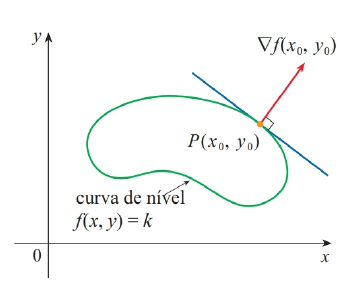
\includegraphics[scale=.6]{figuras/grad1.png}
\end{minipage}\ \ \ \
\begin{minipage}{0.4\textwidth}
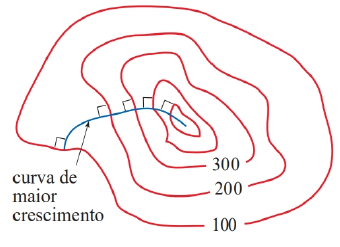
\includegraphics[scale=.6]{figuras/grad2.png}
\end{minipage}
\end{center}
\end{frame}

\subsection*{Teorema da Função Implícita}

\begin{frame}[label=der-parciais]{Diferenciação Implícita}
A função $F(x,y)=x^2+y^2$ tem como curvas de nível círculos centrados na origem.
\[x^2+y^2=k,\ k\geq 0.\]
 Sabemos que o círculo não é o gráfico de uma função de uma variável, entretanto, ao isolarmos uma das variáveis, ele pode ser visto como a união de dois gráficos:
 \[y=\pm\sqrt{k-x^2} \text{ ou } x=\pm\sqrt{k-y^2}\]
Entretanto, na maioria dos casos não é possível isolar uma das variáveis. Nestes casos, como podemos garantir que um pedaço da curva pode ser vista como gráfico de função? Ou dito de outra forma, como garantir que uma variável pode ser colocada em função das demais?
\end{frame}

\begin{frame}[label=der-parciais]{Teorema da Função Implícita I}
Suponha que 
\begin{enumerate}
\item A função $z=F(x,y)$ seja de {\color{blue}classe $C^1$};

\item $F(x_0,y_0)=0$ e ${\color{red}\dy{F}(x_0,y_0)\neq 0}$.
\end{enumerate}
Então, existe uma vizinhança $I$ em torno do ponto $x_0$ e uma {\color{blue}única} função $y=y(x)$ {\color{blue}também de classe $C^1$} tais que 
\[F(x,y(x))=0,\ \text{ para todo } x\in I \]
 e vale
 \[   {\frac{dy}{dx}}=\dps -\frac{\dx{F}}{{\color{red}{\dy{F}}}}.\] 

\begin{exe}
Mostre que $x^3+y^3-6xy=0$ define $y$ como função de $x$ na vizinhança do ponto $(3,3)$ e calcule $y'(3)$ a derivada neste ponto.
\end{exe}

\end{frame}


\begin{frame}[label=der-parciais]{Teorema da Função Implícita II}
Suponha que 
\begin{enumerate}
\item A função $F(x,y,z)$ seja de {\color{blue}classe $C^1$};

\item $F(x_0,y_0,z_0)=0$ e {\color{red}$\dz{F}(x_0,y_0,z_0)\neq 0$}.
\end{enumerate}
Então, existe uma vizinhança $U$ em torno do ponto $(x_0,y_0)$ e uma {\color{blue}única} função $z=z(x,y)$, {\color{blue} também de classe $C^1$}, tais que 
\[F(x,y,z(x,y))=0,\ \text{ para todo } (x,y)\in U \]
 e vale
 \[   \dx{z}=\dps -\frac{\dx{F}}{{\color{red}{\dz{F}}}}\text{ e }   \dy{z}=\dps -\frac{\dy{F}}{{\color{red}{\dz{F}}}}.\] 

%\begin{exe}
%Mostre que $z$ pode ser definida como uma função de $x$ e $y$ na vizinhança de $(0,0)$ para a equação
%\[x^3+z^2+ye^{xz}+z\cos(y)\]
%\end{exe}

\end{frame}


\begin{frame}[label=der-parciais]
\begin{exe}
Verifique que a equação $x^3+3y^2+8xz^2-3z^3y=9$ define $z$ com função de $x$ e $y$ numa vizinhança do ponto $(1,0,1)$ e calcule $\dps\frac{\partial z}{\partial x}(1,0)$, $\dps\frac{\partial z}{\partial y}(1,0)$ e $\dps\frac{\partial^2  z}{\partial y\partial x}(1,0)$.
\end{exe}
\end{frame}


